\section{연구 결과}
이 절의 수치와 그림은 양 다리의 이상적 토크 배분을 사용한 구형 모형의 결과를 보존한 것이다. 3절의 한쪽 활성 다리 및 부담 평탄화 방법으로 재계산한 결과가 아니므로, 새 방법의 개선율이나 검증 결과로 해석하지 않는다.

\subsection{모양을 넓혀 가며 푼 결과}
구형 모형의 볼록 최적화 문제를 조건을 바꿔 가며 풀었던 결과이다(<Table~\ref{tab:conv}>). 부담 감소는 이상적 배분일 때 원형 대비 \(E^\ast\)의 감소율이며, 현재 식 (\ref{eq:opt})의 목적값 감소와 다르다.

\begin{table}[!htb]
\centering\small\renewcommand{\arraystretch}{1.0}
\begin{tabular}{@{}lcccccc@{}}
\toprule
 & \multicolumn{2}{c}{볼록만} & \multicolumn{2}{c}{볼록, 지름비 \(\le2\)} & \multicolumn{2}{c}{곡률반지름 \(\ge0.3\bar\rho\), 지름비 \(\le2\)}\\
\(M\) & 60 / 100 rpm & 지름비 & 60 / 100 rpm & & 60 / 100 rpm & 지름비\\\midrule
2 & 1.69 / 3.09 & 2.00 & 1.69 / 3.09 & & 1.31 / 2.41 & 1.61\\
4 & 2.12 / 3.87 & 2.90 & 1.72 / 3.15 & & 1.71 / 3.12 & 2.00\\
8 & 2.38 / 4.33 & 4.67 & 1.74 / 3.19 & & 1.71 / 3.14 & 2.00\\
12 & 2.45 / 4.47 & 6.36 & 1.79 / 3.27 & & 1.75 / 3.20 & 2.00\\
24 & 2.51 / 4.57 & 10.1 & 1.81 / 3.32 & & 1.78 / 3.25 & 2.00\\
점 720개 & 2.55 / 4.63 & 26.2 & 1.82 / 3.34 & & 1.79 / 3.27 & 2.00\\\midrule
제약 없음, 구형 모형의 해석해 & \multicolumn{6}{l}{2.60 / 4.72 (오목한 곳이 있어 만들 수 없음)}\\
\bottomrule
\end{tabular}
\caption{조건과 푸리에 차수 \(M\)에 따른 부담 감소율 (\%)}
\label{tab:conv}
\end{table}

\begin{enumerate}
\item \textbf{홀수 성분.} 홀수 계수(\(n=1,3,\dots\))는 막지 않았는데도 모든 경우에 \(10^{-5}\bar\rho\) 아래로 나왔다. \(K(\theta+\pi)=K(\theta)\)이고 볼록 문제의 최적은 하나뿐이므로, 최적 모양을 \(180^\circ\) 돌린 것도 최적이어서 둘이 같아야 하기 때문이다. 그래서 위아래 체인 줄이 나란하면 \(\rho_-(\theta)=\rho_+(\theta+\pi)=\rho_+(\theta)\)가 정확히 성립한다.
\item \textbf{제작 조건이 없으면.} 구형 모형에서 볼록 조건만 두면 \(M\)을 키울수록 지름비가 끝없이 커지고, 점 720개로 풀면 지름비 26의 가늘고 모서리가 있는 모양이 된다. 효과는 구형 모형의 해석적 상한에 거의 닿지만 만들 수 없으므로, 지름비와 곡률반지름 조건을 두었다.
\item \textbf{현실적인 조건에서는.} \(M=2\)(이론 문서의 \(\cos2\theta\) 한 성분 꼴)는 곡률 조건 때문에 지름비가 1.61에서 막혀 효과가 작다. \(M=4\)에서 \(\cos4\theta\) 성분이 긴 축 끝을 둥글게 만들어 지름비 2를 다 쓸 수 있게 되고, 그 뒤로는 \(M=24\)까지 넓혀도 0.07--0.13\%p만 늘어난다.
\end{enumerate}

\subsection{결과 체인링}
<Table~\ref{tab:result}>는 지름비 2인 모양들의 비교이다. 타원은 \(\cos2\theta\)에 작은 \(\cos4\theta\)가 섞인 모양이라 푸리에 \(M=4\)의 최적과 0.03\%p 이내로 같고, 식이 간단하다. 한 성분 꼴은 \(e=1/3\)에서 긴 축 끝의 곡률반지름이 0이 되지만 타원은 26.9 mm이다. 효과가 가장 큰 방향(\(\theta_M=135.8^\circ\))에서는 데드스팟 직후 \(T_+<0\)이 되므로, 붙이는 각도를 \(6^\circ\) 당긴 \(\theta_M=129.8^\circ\)의 타원을 결과 체인링으로 정하였다. 효과는 0.06--0.11\%p 줄지만 두 케이던스 모두 한 바퀴 내내 \(T_+>0\)이다.

\begin{table}[!htb]
\centering\small\renewcommand{\arraystretch}{1.0}
\begin{tabular}{@{}lccccc@{}}
\toprule
모양 & 최소 곡률반지름 & \multicolumn{2}{c}{부담 감소 (\%)} & \multicolumn{2}{c}{\(T_+\) 최솟값 (N)}\\
 & (mm) & 60 rpm & 100 rpm & 60 rpm & 100 rpm\\\midrule
원형 & 83.0 & 기준 & 기준 & 7 & \(-4\)\\
\(\bar\rho[1+e\cos2(\theta-\theta_M)]\), \(e=1/3\) & 0 & 1.69 & 3.09 & \(-30\) & \(-115\)\\
푸리에 \(M=4\) & 24.9 & 1.71 & 3.12 & \(-40\) & \(-144\)\\
푸리에 \(M=24\) & 24.9 & 1.78 & 3.25 & 1 & \(-230\)\\
타원, \(\theta_M=135.8^\circ\) & 26.9 & 1.69 & 3.10 & \(-44\) & \(-155\)\\
\textbf{타원, \(\theta_M=129.8^\circ\) (결과)} & 26.9 & \textbf{1.63} & \textbf{2.99} & \textbf{23} & \textbf{31}\\
\bottomrule
\end{tabular}
\caption{지름비 2인 체인링 모양별 결과 (원형만 지름비 1)}
\label{tab:result}
\end{table}

\begin{figure}[!htb]
\centering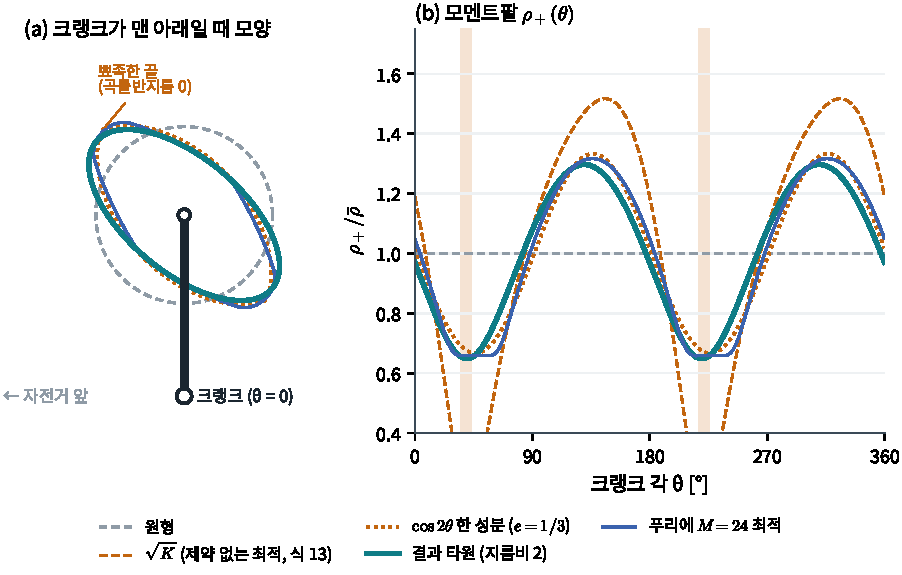
\includegraphics[width=0.85\textwidth]{f_shapes.pdf}
\caption{구형 모형의 결과 체인링. (a) 크랭크가 맨 아래일 때의 피치곡선. 한 성분 꼴은 \(e=1/3\)에서 긴 축 끝이 뾰족해진다. (b) 모멘트팔. 구형 모형의 제약 없는 형상은 \(\sqrt K\)를 따른다.}
\label{fig:shapes}
\end{figure}

구형 모형에서는 원형이 100 rpm에서 \(T_+\)가 음수가 되는 구간을 보였다. 당시의 장력 보정 기준으로 비교한 원형의 부담은 100 rpm에서 0.243이 아니라 0.342였고, 결과 체인링은 0.236이었다. 이 값은 현재의 요구 토크 기반 부담과 다른 지표이며 새 모형에 그대로 적용하지 않는다.

[Fig.~\ref{fig:film}]는 결과 체인링이 반 바퀴 도는 모습이다. 모멘트팔이 가장 큰 \(\theta\approx130^\circ\)에서 크랭크는 평균보다 23\% 느리게 돌고, 데드스팟(\(39^\circ\))은 54\% 빠르게 지나간다.

\begin{figure}[!htb]
\centering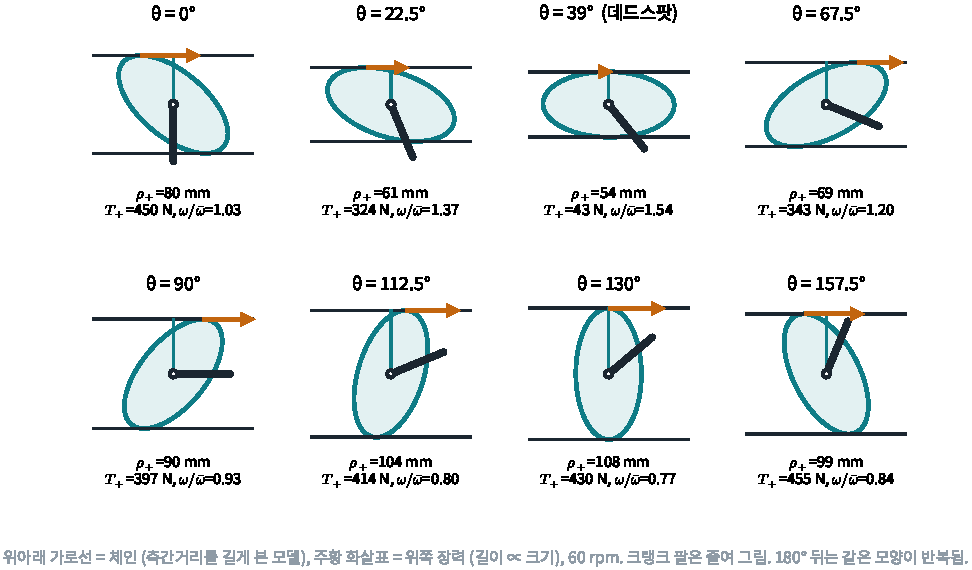
\includegraphics[width=0.9\textwidth]{f_film.pdf}
\caption{결과 체인링이 반 바퀴 도는 동안의 모멘트팔, 위쪽 장력, 크랭크 빠르기 (60 rpm). 주황 화살표의 길이는 장력에 비례한다.}
\label{fig:film}
\end{figure}

\subsection{모델 안의 힘}
[Fig.~\ref{fig:drive}]는 결과 체인링의 한 순간(\(60\) rpm, \(\theta=260^\circ\)) 힘을 실제 비율로 그린 것이다. 오른다리는 정강이 방향으로 142 N을 밀고, 이 중 크랭크에 수직인 성분은 109 N, 크랭크 방향 성분은 91 N이다. 왼다리는 올라가는 중이라 페달을 152 N으로 당긴다. 두 다리의 크랭크 토크는 \(18.5+11.0=29.5\) N\(\cdot\)m이고, 위쪽 장력 383 N이 만드는 토크는 \(0.0807\times383=30.9\) N\(\cdot\)m이다. 그 차이 \(-1.5\) N\(\cdot\)m가 이 순간 크랭크와 다리의 운동에너지 변화 \(\frac{d}{d\theta}(\frac12J\omega^2)\)이다. 체인은 링을 뒤로 당기므로 축 반력(337 N)은 앞을 향한다.

\begin{figure}[!htb]
\centering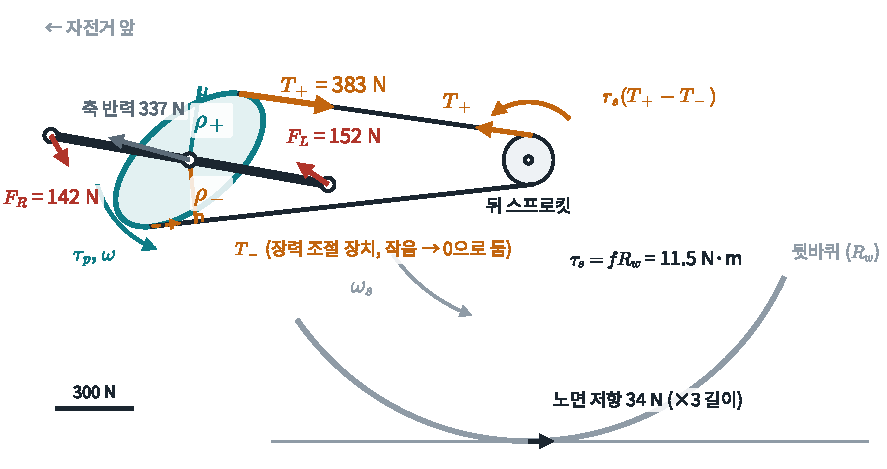
\includegraphics[width=0.85\textwidth]{f_drive.pdf}
\caption{구동계에 걸리는 힘 (결과 체인링, \(60\) rpm, \(\theta=260^\circ\)). 빨강: 정강이가 페달에 주는 힘, 주황: 체인 장력, 회색: 축 반력. 노면 저항은 길이를 3배로 그렸다.}
\label{fig:drive}
\end{figure}

[Fig.~\ref{fig:curves}]는 한 바퀴 동안의 힘이다. 각도별 페달 힘의 방향과 크기는 원형과 결과 체인링이 거의 같은데, 힘의 방향은 정강이 방향이 정하기 때문이다. 위쪽 장력은 원형이 60 rpm에서 7--598 N, 100 rpm에서 \(-4\)--532 N으로 크게 변하고, 결과 체인링은 23--458 N, 31--278 N으로 변동폭이 작다.

\begin{figure}[!htb]
\centering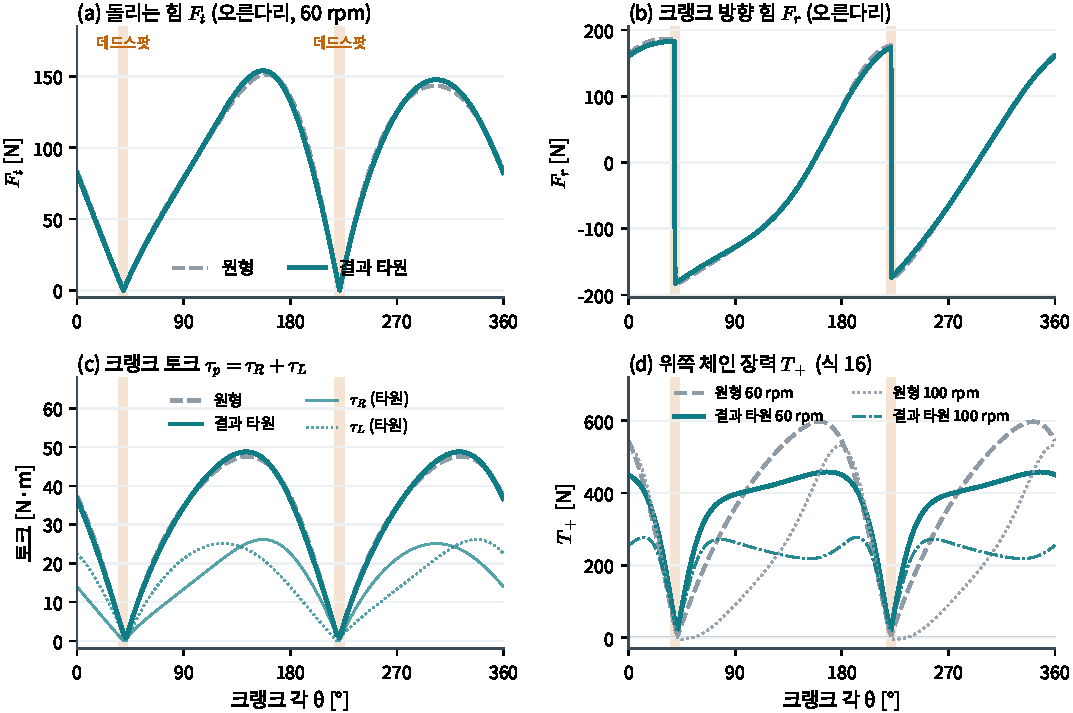
\includegraphics[width=0.9\textwidth]{f_curves.pdf}
\caption{구형 모형에서 계산한 크랭크 각에 따른 힘. (a), (b) 오른다리 페달 힘의 두 성분. (c) 두 다리의 크랭크 토크와 합. (d) 당시의 동역학 식으로 구한 위쪽 체인 장력. 주황 띠는 데드스팟이다.}
\label{fig:curves}
\end{figure}

\subsection{효과 지수}
선행연구의 효과 지수\cite{candotti2007,bini2013}를 우리 모델에 적용하였다. 오른다리의 페달 힘으로 시간에 대해 평균하면
\begin{equation}
\mathrm{IE}=\frac{\int F_t\,dt}{\int |F|\,dt}=\frac{\oint F_t/\omega\,d\theta}{\oint |F|/\omega\,d\theta} \label{eq:16}
\end{equation}
이고, 결과는 <Table~\ref{tab:ie}>와 같다. 결과 체인링은 모든 케이던스에서 IE가 약 0.07 크다. 그러나 각도마다 같은 가중치로 평균하면 원형 0.583, 결과 0.589로 거의 같다. 차이는 데드스팟 \(\pm10^\circ\) 안에 머무는 시간이 한 바퀴의 11.0\%에서 7.3\%로 줄어든 데서 온다([Fig.~\ref{fig:clock}]).

\begin{table}[!htb]
\centering\small
\begin{tabular}{@{}lcccc@{}}
\toprule
케이던스 (rpm) & 40 & 60 & 80 & 100\\\midrule
원형 & 0.590 & 0.583 & 0.576 & 0.568\\
결과 체인링 & 0.658 & 0.654 & 0.649 & 0.644\\
\bottomrule
\end{tabular}
\caption{오른다리 페달 힘의 효과 지수 (식 (\ref{eq:16}))}
\label{tab:ie}
\end{table}

\begin{figure}[!htb]
\centering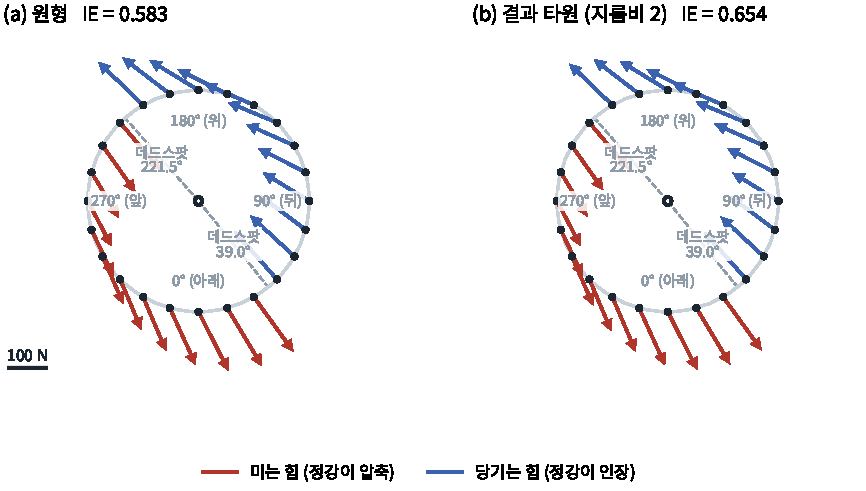
\includegraphics[width=0.9\textwidth]{f_clock.pdf}
\caption{오른쪽 페달에 걸리는 힘 (\(60\) rpm, \(15^\circ\) 간격). 아래쪽 반 바퀴는 밀고 위쪽 반 바퀴는 당긴다.}
\label{fig:clock}
\end{figure}
